\documentclass[10pt]{article}

\usepackage[utf8]{inputenc}
\usepackage[spanish]{babel}
\decimalpoint
\usepackage{amsmath, amssymb}
\usepackage{xcolor}
\usepackage{geometry}
\geometry{letterpaper, margin=1in}
\usepackage{graphicx}
\usepackage{float}
\usepackage{array}
\usepackage{booktabs}
\usepackage{colortbl}
\usepackage{caption}
\usepackage{tocloft}

\usepackage[colorlinks=true, linkcolor=black, urlcolor=black, citecolor=black]{hyperref}
%%%%%%%%%%%%%%%%%%%%%%%%%%%%%%%%%%%%%%%%%%%%%%%%%%%%%%%%%%%%%%%%%%%%%%%%%%%%%%%%%%%%%%%%%%%%%%%%%%%%%%%%%%%%%%
%%%%%%%%%%%%%%%%%%%%%%%%%%%%%%%%%%%%%%%%%%%%%%%%%%%%%%%%%%%%%%%%%%%%%%%%%%%%%%%%%%%%%%%%%%%%%%%%%%%%%%%%%%%%%%
\title{Universidad Panamericana \\ Maestría en Ciencia de Datos \\ Datos Masivos \\ 
    \vspace{0.5cm} Proyecto Final: \textit{Monitoreo Inteligente de Tráfico Marítimo con Big Data AIS}}
\author{Enrique Ulises Báez Gómez Tagle, Luis Alejandro Guillén Alvarez}
\date{\today}
%%%%%%%%%%%%%%%%%%%%%%%%%%%%%%%%%%%%%%%%%%%%%%%%%%%%%%%%%%%%%%%%%%%%%%%%%%%%%%%%%%%%%%%%%%%%%%%%%%%%%%%%%%%%%%
%%%%%%%%%%%%%%%%%%%%%%%%%%%%%%%%%%%%%%%%%%%%%%%%%%%%%%%%%%%%%%%%%%%%%%%%%%%%%%%%%%%%%%%%%%%%%%%%%%%%%%%%%%%%%%
%%%%%%%%%%%%%%%%%%%%%%%%%%%%%%%%%%%%%%%%%%%%%%%%%%%%%%%%%%%%%%%%%%%%%%%%%%%%%%%%%%%%%%%%%%%%%%%%%%%%%%%%%%%%%%%%%%%%%%%%%%%%%%%%%%%%%%%%%%%%%%%%%%%%%%%%%%%%%%%%%%%%%%%%%%%%%%%%%%%%%%%%%%%%%%
%%%%%%%%%%%%%%%%%%%%%%%%%%%%%%%%%%%%%%%%%%%%%%%%%%%%%%%%%%%%%%%%%%%%%%%%%%%%%%%%%%%%%%%%%%%%%%%%%%%%%%%%%%%%%%%%%%%%%%%%%%%%%%%%%%%%%%%%%%%%%%%%%%%%%%%%%%%%%%%%%%%%%%%%%%%%%%%%%%%%%%%%%%%%%%
\begin{document}

\maketitle

\tableofcontents

\newpage

%%%%%%%%%%%%%%%%%%%%%%%%%%%%%%%%%%%%%%%%%%%%%%%%%%%%%%%%%%%%%%%%%%%%%%%%%%%%%%%%%%%%%%%%%%%%%%%%%%%%%%%%%%%%%%%%%%%%%%%%%%%%%%%%%%%%%%%%%%%%%%%%%%%%%%%%%%%%%%%%%%%%%%%%%%%%%%%%%%%%%%%%%%%%%%
%%%%%%%%%%%%%%%%%%%%%%%%%%%%%%%%%%%%%%%%%%%%%%%%%%%%%%%%%%%%%%%%%%%%%%%%%%%%%%%%%%%%%%%%%%%%%%%%%%%%%%%%%%%%%%%%%%%%%%%%%%%%%%%%%%%%%%%%%%%%%%%%%%%%%%%%%%%%%%%%%%%%%%%%%%%%%%%%%%%%%%%%%%%%%%
\section{Resumen ejecutivo}
\subsection{Introducción} % REVISIÓN GUILLÉN 

El tráfico marítimo global genera millones de registros de posicionamiento a través del Sistema de Identificación Automática (AIS), que transmite automáticamente la identidad, posición, velocidad y otros datos de los buques. Originalmente implementado para mejorar la seguridad de la navegación, hoy es crucial para la gestión del tráfico marítimo, la conciencia del entorno y operaciones de búsqueda y rescate.

Este proyecto propone aprovechar Big Data y aprendizaje automático (ML) para analizar una base de datos masiva de mensajes AIS y ofrecer una solución innovadora a la pregunta: \textbf{¿Cómo detectar y entender comportamientos anómalos en el tráfico marítimo para mejorar la seguridad y la eficiencia?}

Responder esta pregunta implica analizar patrones normales de navegación y descubrir desviaciones significativas. En esencia:
\begin{itemize}
    \item \textbf{¿Qué estamos haciendo?} Diseñamos un sistema de análisis que procesa grandes volúmenes de datos AIS para identificar anomalías en el comportamiento de los buques (posiciones fuera de lugar, velocidades inusuales, maniobras erráticas, etc.) y extraer patrones útiles sobre la operación de diferentes tipos de embarcaciones.
    \item \textbf{¿Para qué lo hacemos?} Para mejorar la seguridad marítima, la gestión del tráfico y la toma de decisiones, ofreciendo alertas tempranas de potenciales riesgos (colisiones, actividades ilícitas o fallos) y conocimiento profundo a autoridades y empresas navieras.
    \item \textbf{¿Cómo lo hacemos?} Empleando herramientas de Big Data de la Suite de Google Cloud (Storage + DataProc + BigQuery) para procesar datos geoespaciales masivos en en poco tiempo, complementado con modelos de ML que aprenden patrones habituales y detectan comportamientos que se apartan de lo normal.
    \item \textbf{¿A quién beneficia?} A organismos de seguridad marítima (marinas, guardacostas), a empresas navieras optimizando rutas y monitoreo de flotas, a aseguradoras evaluando riesgos operativos e incluso a investigadores del medio marino en estudios ecológicos.
\end{itemize}

Finalmente, los resultados se integraron en un \textit{dashboard} interactivo con visualizaciones (mapas geográficos, gráficos de tendencias y rankings) que facilitan la interpretación y la toma de decisiones.
%%%%%%%%%%%%%%%%%%%%%%%%%%%%%%%%%%%%%%%%%%%%%%%%%%%%%%%%%%%%%%%%%%%%%%%%%%%%%%%%%%%%%%%%%%%%%%%%%%%%%%%%%%%%%%%%%%%%%%%%%%%%%%%%%%%%%%%%%%%%%%%%%%%%%%%%%%%%%%%%%%%%%%%%%%%%%%%%%%%%%%%%%%%%%%
%%%%%%%%%%%%%%%%%%%%%%%%%%%%%%%%%%%%%%%%%%%%%%%%%%%%%%%%%%%%%%%%%%%%%%%%%%%%%%%%%%%%%%%%%%%%%%%%%%%%%%%%%%%%%%%%%%%%%%%%%%%%%%%%%%%%%%%%%%%%%%%%%%%%%%%%%%%%%%%%%%%%%%%%%%%%%%%%%%%%%%%%%%%%%%
\section{Visión general del desarrollo} 
\subsection{Solución Actual / visión general} % REVISIÓN GUILLÉN: FALTA AÑADIR PARTE DE ML tanto descripción como diagrama

La solución actual se implementa de extremo a extremo sobre la nube de Google Cloud. El flujo completo es el siguiente:

\begin{itemize}
    \item Una máquina virtual en Google Compute Engine se encarga de \textbf{scrapear los datos AIS} y cargarlos en Google Cloud Storage. 
    \item En Cloud Storage se organizan dos capas diferenciadas: \textit{raw} y \textit{curated}, con prefijos de carpeta y particiones por mes (\texttt{YYYY-MM=}).
    \item Un clúster de Google Cloud DataProc (perfil \emph{high-memory}; véase Sección~\ref{sec:cluster}) ejecuta dos jobs, habilitando procesamientos por series de meses con menos derrames a disco y menor tiempo total:
    \begin{itemize}
        \item Job \textbf{raw}: descomprime los archivos obtenidos y organiza los datos en particiones por año y mes, y finalmente los guarda en formato Parquet en Google Cloud Storage.
        \item Job \textbf{curated}: lee la capa cruda, aplica transformaciones iniciales y genera la capa refinada lista para análisis.
    \end{itemize}
    \item Una Cloud Function crea el \textbf{dataset y la tabla en BigQuery}, cargando la información desde la capa curated.
    \item En BigQuery se centraliza la explotación de datos mediante consultas SQL optimizadas, generando los datasets finales que alimentan las visualizaciones.
    \item El \textbf{dashboard de Streamlit}, desplegado en la misma VM, consume los resultados de BigQuery y presenta mapas, gráficos de tendencias y rankings de manera interactiva.
\end{itemize}

\vspace{0.5cm}
\begin{figure}[H]
    \centering
    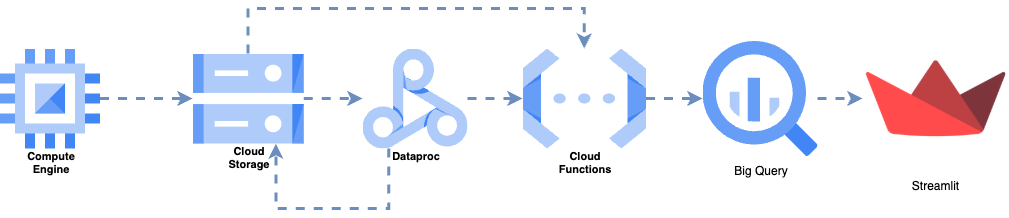
\includegraphics[width=\textwidth]{figures/arch/ArchitectureDiagram.png}
    \caption{Arquitectura actual de la solución: flujo end-to-end en Google Cloud.}
\end{figure}
\vspace{0.1cm}
%%%%%%%%%%%%%%%%%%%%%%%%%%%%%%%%%%%%%%%%%%%%%%%%%%%%%%%%%%%%%%%%%%%%%%%%%%%%%%%%%%%%%%%%%%%%%%%%%%%%%%%%%%%%%%%%%%%%%%%%%%%%%%%%%%%%%%%%%%%%%%%%%%%%%%%%%%%%%%%%%%%%%%%%%%%%%%%%%%%%%%%%%%%%%%
%%%%%%%%%%%%%%%%%%%%%%%%%%%%%%%%%%%%%%%%%%%%%%%%%%%%%%%%%%%%%%%%%%%%%%%%%%%%%%%%%%%%%%%%%%%%%%%%%%%%%%%%%%%%%%%%%%%%%%%%%%%%%%%%%%%%%%%%%%%%%%%%%%%%%%%%%%%%%%%%%%%%%%%%%%%%%%%%%%%%%%%%%%%%%%
\subsection{Limitaciones actuales de la solución}
\label{subsec:limitaciones-solucion}

\begin{itemize}
  \item \textbf{Sin orquestación event-driven.} Los disparadores son manuales o programados; la activación automática por eventos de GCS/Pub\,\/Sub o Workflows aún no está implementada. Migrar a un esquema event-driven reduciría intervención manual y tiempos de ciclo.
  \item \textbf{No tiempo real.} El pipeline es \textit{batch}; no hay ingesta en streaming ni SLA de latencia. El dashboard refleja cortes al cierre de cada corrida.
  \item \textbf{Evolución de esquema limitada.} La Cloud Function crea tablas y puede autodetectar esquema, pero no hay un proceso formal de migraciones/versionado ni \textit{backfills} automatizados.
  \item \textbf{Pruebas y monitoreo.} Podrían generarse alertas proactivas (Cloud Monitoring/Error Reporting) ante fallas o derivas.
\end{itemize}

%%%%%%%%%%%%%%%%%%%%%%%%%%%%%%%%%%%%%%%%%%%%%%%%%%%%%%%%%%%%%%%%%%%%%%%%%%%%%%%%%%%%%%%%%%%%%%%%%%%%%%%%%%%%%%%%%%%%%%%%%%%%%%%%%%%%%%%%%%%%%%%%%%%%%%%%%%%%%%%%%%%%%%%%%%%%%%%%%%%%%%%%%%%%%%
%%%%%%%%%%%%%%%%%%%%%%%%%%%%%%%%%%%%%%%%%%%%%%%%%%%%%%%%%%%%%%%%%%%%%%%%%%%%%%%%%%%%%%%%%%%%%%%%%%%%%%%%%%%%%%%%%%%%%%%%%%%%%%%%%%%%%%%%%%%%%%%%%%%%%%%%%%%%%%%%%%%%%%%%%%%%%%%%%%%%%%%%%%%%%%
\subsection{Propósito, uso y alcance de la herramienta} % TODO: GUILLÉN
%%%%%%%%%%%%%%%%%%%%%%%%%%%%%%%%%%%%%%%%%%%%%%%%%%%%%%%%%%%%%%%%%%%%%%%%%%%%%%%%%%%%%%%%%%%%%%%%%%%%%%%%%%%%%%%%%%%%%%%%%%%%%%%%%%%%%%%%%%%%%%%%%%%%%%%%%%%%%%%%%%%%%%%%%%%%%%%%%%%%%%%%%%%%%%
\section{Revisión y uso de datos}
\subsection{Orígenes y control de datos} % REVISIÓN GUILLÉN

Los datos utilizados provienen del portal oficial de la NOAA (\url{https://coast.noaa.gov/htdata/CMSP/AISDataHandler/2024/index.html}), el cual publica archivos comprimidos (.zip) con los mensajes AIS recolectados a lo largo del año 2024. 
Para garantizar la trazabilidad y el control de los datos, se desarrolló un script en Python (\texttt{scrapper.py}) que automatiza la descarga de todos los archivos disponibles, verificando duplicados mediante el tamaño de los ficheros y evitando descargas innecesarias. 
De esta manera se asegura que la totalidad de los datos originales publicados por la NOAA sean capturados sin alteración.

%%%%%%%%%%%%%%%%%%%%%%%%%%%%%%%%%%%%%%%%%%%%%%%%%%%%%%%%%%%%%%%%%%%%%%%%%%%%%%%%%%%%%%%%%%%%%%%%%%%%%%%%%%%%%%%%%%%%%%%%%%%%%%%%%%%%%%%%%%%%%%%%%%%%%%%%%%%%%%%%%%%%%%%%%%%%%%%%%%%%%%%%%%%%%%
\subsection{Preparación de datos} % REVISIÓN GUILLÉN
En esta sección se describe el \textbf{qué} produce la preparación de datos (entradas, salidas y \emph{esquema}); la orquestación y operación del pipeline (el \textbf{cómo}) se documenta en la Sección~\ref{sec:metodologia}.

La preparación de los datos comienza en una máquina virtual de Google Compute Engine, donde se ejecuta el script de \textit{scraping}. Este proceso descarga en paralelo (con \textit{threads}) los archivos \texttt{.zip} hacia un directorio local (\texttt{ais\_2024}) y posteriormente los traslada a Google Cloud Storage en la capa \textbf{raw}.\\

Dado el objetivo de tener un conjunto uniforme, trazable y listo para análisis, con: (i) esquema estandarizado, (ii) claves y derivadas temporales consistentes, (iii) coordenadas y velocidades normalizadas, y (iv) datos particionados por \texttt{ym} (AAAA-MM).

\paragraph{Entradas $\rightarrow$ salidas por etapa y la salida de cada una.}
\begin{enumerate}
  \item \textbf{RAW INGESTION}: entrada = lotes \texttt{.zip} de NOAA; salida = archivos Parquet en \textbf{raw} \emph{particionados por \texttt{ym}}, con trazabilidad mínima (archivo fuente y timestamp de ingesta).
  \item \textbf{CURATED TRANSFORMATIONS}: entrada = \textbf{raw}; salida = capa \textbf{curated} con tipos normalizados, derivados temporales y desduplicación por \texttt{MMSI+BaseDateTime}. Las reglas de limpieza y validaciones se detallan en la Sección~\ref{sec:cleaning}.
\end{enumerate}

\paragraph{Modelo de datos de la capa \textit{curated}.}
El Cuadro~\ref{tab:curated_schema} presenta los campos principales que expone la capa analítica.

\begin{table}[H]
  \centering
  \caption{Esquema de la capa \textit{curated}.}
  \label{tab:curated_schema}
  \scriptsize
  \begin{tabular}{@{}llp{8cm}@{}}
  \toprule
  Campo & Tipo & Descripción \\
  \midrule
  NavStatusInt & INTEGER & Representación entera del estado de navegación del buque. \\
  MMSI & STRING & Número de Identidad del Servicio Móvil Marítimo del buque. \\
  BaseDateTime & TIMESTAMP & Marca temporal que indica la fecha y hora del mensaje AIS. \\
  LAT & FLOAT & Latitud de la posición del buque. \\
  LON & FLOAT & Longitud de la posición del buque. \\
  SOG & FLOAT & Velocidad sobre el fondo del buque en nudos. \\
  COG & FLOAT & Rumbo sobre el fondo del buque en grados. \\
  Heading & FLOAT & Rumbo de la proa del buque en grados. \\
  VesselName & STRING & Nombre del buque. \\
  IMO & STRING & Número de la Organización Marítima Internacional del buque. \\
  CallSign & STRING & Indicativo de llamada por radio del buque. \\
  VesselType & STRING & Tipo de buque. \\
  Status & STRING & Estado del buque. \\
  Length & FLOAT & Eslora del buque. \\
  Width & FLOAT & Manga del buque. \\
  Draft & FLOAT & Calado del buque. \\
  Cargo & STRING & Tipo de carga que transporta el buque. \\
  TransceiverClass & STRING & Clase del transpondedor AIS. \\
  \_source\_file & STRING & Nombre del archivo fuente desde el cual se ingirieron los datos. \\
  \_ingest\_ts & TIMESTAMP & Marca temporal que indica cuándo se ingirieron los datos en la tabla. \\
  ymd & STRING & Fecha en formato año-mes-día. \\
  VesselTypeInt & INTEGER & Representación entera del tipo de buque. \\
  VesselTypeCode & STRING & Código que representa el tipo de buque. \\
  VesselTypeName & STRING & Nombre del tipo de buque. \\
  VesselTypeClass & STRING & Clasificación del tipo de buque. \\
  NavStatusName & STRING & Nombre del estado de navegación del buque. \\
  date & DATE & Fecha en que se registró el mensaje AIS. \\
  hour & INTEGER & Hora del día en que se registró el mensaje AIS. \\
  dow & STRING & Día de la semana en que se registró el mensaje AIS. \\
  week & INTEGER & Semana del año en que se registró el mensaje AIS. \\
  month & INTEGER & Mes en que se registró el mensaje AIS. \\
  quarter & INTEGER & Trimestre del año en que se registró el mensaje AIS. \\
  SOG\_ms & FLOAT & Velocidad sobre el fondo del buque en metros por segundo. \\
  geohash9 & STRING & Representación geohash de la posición del buque con precisión de 9 caracteres. \\
  \bottomrule
  \end{tabular}
\end{table}

Una vez procesado, el resultado de este pipeline se publica en BigQuery como tabla particionada por \texttt{ym}, optimizada para consulta y consumo por el \textit{dashboard}. Los detalles de automatización de creación/carga (Cloud Function, idempotencia y autodetección de esquema) se abordan en la Sección~\ref{sec:metodologia}.
%%%%%%%%%%%%%%%%%%%%%%%%%%%%%%%%%%%%%%%%%%%%%%%%%%%%%%%%%%%%%%%%%%%%%%%%%%%%%%%%%%%%%%%%%%%%%%%%%%%%%%%%%%%%%%%%%%%%%%%%%%%%%%%%%%%%%%%%%%%%%%%%%%%%%%%%%%%%%%%%%%%%%%%%%%%%%%%%%%%%%%%%%%%%%%
\subsection{Limpieza y tratamiento de datos} % REVISIÓN GUILLÉN 
\label{sec:cleaning}

En esta sección se describen de manera detallada las transformaciones y criterios aplicados para convertir los datos AIS en una capa \textbf{curated} funcional para el análisis. Se listan los pasos con su \emph{porqué} operativo o estadístico.

\paragraph{Normalizaciones y tipos.}
\begin{itemize}
  \item \textbf{Casteo y estandarización}: se convierten columnas numéricas a tipos adecuados (\texttt{double}/\texttt{int}) y se normalizan textos (\texttt{trim}, mayúsculas controladas) para evitar variabilidad en joins/agrupaciones.
  \item \textbf{Timestamps en UTC}: \texttt{BaseDateTime} se parsea a tipo timestamp con zona UTC para análisis temporales coherentes; sobre esta base se derivan \texttt{date}, \texttt{hour}, \texttt{week}, \texttt{month}, \texttt{quarter} y una columna \texttt{ym} (AAAA-MM) para particionado.
\end{itemize}

\paragraph{Coordenadas y límites físicos.}
\begin{itemize}
  \item \textbf{LAT/LON válidos}: se recortan latitudes al rango [-90, 90] y longitudes se \emph{envuelven} a [-180, 180] (corrigiendo valores fuera de dominio por errores/reporte). Se descartan registros con coordenadas nulas tras la corrección.
  \item \textbf{Redondeo razonable}: se redondean LAT/LON a 5 decimales para homogenizar precisión sin perder resolución náutica relevante.
\end{itemize}

\paragraph{Velocidad, rumbos y estados.}
\begin{itemize}
  \item \textbf{SOG (Speed Over Ground)}: se acota a [0, 70] nudos para eliminar outliers físicos/telemetría corrupta; adicionalmente se calcula \texttt{SOG\_ms} en m/s para modelos.
  \item \textbf{COG/Heading}: se normaliza módulo 360°. El valor \texttt{Heading=511} (no disponible) se marca como nulo para evitar sesgos en métricas de rumbo.
  \item \textbf{NavStatus}: se genera \texttt{NavStatusInt} a partir de \texttt{Status} y se une contra un catálogo para \texttt{NavStatusName}; códigos fuera de 0–15 se etiquetan como \textit{Unknown} y faltantes como \textit{Not reported}.
\end{itemize}

\paragraph{Dimensiones y calado.}
\begin{itemize}
  \item \textbf{Length/Width}: se acotan a rangos plausibles (1–450 m y 1–70 m, respectivamente) para descartar errores de orden de magnitud.
  \item \textbf{Draft}: se limita a [0, 25] m; valores negativos o excesivos suelen provenir de carga mal reportada o errores de parsing.
\end{itemize}

\paragraph{Identificadores y texto.}
\begin{itemize}
  \item \textbf{MMSI}: se extrae la porción numérica válida (1–9 dígitos) y se rellena a 9 con ceros a la izquierda para formato consistente.
  \item \textbf{IMO/CallSign/VesselName}: se normalizan espacios y caracteres no alfanuméricos; se limpian IMOs genéricos (p.ej., \texttt{IMO0000000}, \texttt{0}, vacío) para evitar falsas uniones.
\end{itemize}

\paragraph{Clasificación de tipo de buque.}
\begin{itemize}
  \item \textbf{VesselType}: se derivan \texttt{VesselTypeInt}, \texttt{VesselTypeName} (mediante mapa IMO) y \texttt{VesselTypeClass} (WIG, Cargo, Tanker, Passenger, etc.). Esto permite comparar métricas por clase homogénea y soportar reglas dependientes del tipo.
\end{itemize}

\paragraph{Enriquecimiento geoespacial.}
\begin{itemize}
  \item \textbf{Geohash9}: se calcula un \texttt{geohash9} distribuido (UDF con \texttt{pygeohash}) para agregación espacial eficiente y enlaces a capas geográficas (vallas, puertos, TSS) en análisis posteriores.
\end{itemize}

\paragraph{Calidad e idempotencia.}
\begin{itemize}
  \item \textbf{Desduplicación}: se eliminan duplicados por clave compuesta \texttt{(MMSI, BaseDateTime)} para asegurar series temporales limpias por embarcación.
  \item \textbf{Validación de conteos}: en \textit{raw}, se comparan conteos diarios (CSV vs Parquet) y se aborta si no coinciden; en \textit{curated}, se escriben marcadores de éxito por partición (\texttt{\_markers/ym=.../\_SUCCESS}) para reanudación y ejecución incremental sin sobrescribir trabajo correcto.
\end{itemize}
%%%%%%%%%%%%%%%%%%%%%%%%%%%%%%%%%%%%%%%%%%%%%%%%%%%%%%%%%%%%%%%%%%%%%%%%%%%%%%%%%%%%%%%%%%%%%%%%%%%%%%%%%%%%%%%%%%%%%%%%%%%%%%%%%%%%%%%%%%%%%%%%%%%%%%%%%%%%%%%%%%%%%%%%%%%%%%%%%%%%%%%%%%%%%%
\subsection{Integridad de los datos} % TODO: GUILLÉN
%%%%%%%%%%%%%%%%%%%%%%%%%%%%%%%%%%%%%%%%%%%%%%%%%%%%%%%%%%%%%%%%%%%%%%%%%%%%%%%%%%%%%%%%%%%%%%%%%%%%%%%%%%%%%%%%%%%%%%%%%%%%%%%%%%%%%%%%%%%%%%%%%%%%%%%%%%%%%%%%%%%%%%%%%%%%%%%%%%%%%%%%%%%%%%
\subsection{Limitaciones de los datos} % TODO: GUILLÉN
%%%%%%%%%%%%%%%%%%%%%%%%%%%%%%%%%%%%%%%%%%%%%%%%%%%%%%%%%%%%%%%%%%%%%%%%%%%%%%%%%%%%%%%%%%%%%%%%%%%%%%%%%%%%%%%%%%%%%%%%%%%%%%%%%%%%%%%%%%%%%%%%%%%%%%%%%%%%%%%%%%%%%%%%%%%%%%%%%%%%%%%%%%%%%%
\section{Proceso de desarrollo}
\subsection{Metodología} % REVISIÓN GUILLÉN 
\label{sec:metodologia}

Esta sección cubre el \textbf{cómo} se ejecuta y opera el pipeline (orquestación, confiabilidad, despliegue y costos); las reglas de transformación y el esquema se tratan en las Secciones~\ref{sec:cleaning} y \ref{tab:curated_schema}.
\paragraph{Proceso de desarrollo.}
\begin{itemize}
  \item \textbf{Ejecución y calendarización}: actualmente los disparadores son manuales o programados; aún no se emplea un flujo completamente \emph{event-driven} (ver Sección~\ref{subsec:limitaciones-solucion}). 
  \item \textbf{Orquestación y repetibilidad}: los jobs se ejecutan en DataProc con tolerancia a fallos (speculation, retries) e \emph{idempotencia} (sobrescritura controlada por partición y marcadores \texttt{\_SUCCESS}). Esto permite relanzar sin duplicados ni corrupción de particiones.
  \item \textbf{Publicación a BigQuery}: una Cloud Function idempotente verifica/crea \textbf{datasets} y \textbf{tablas}; si no hay esquema, lo autodetecta a partir de una muestra en GCS. Su objetivo es que la capa \textit{curated} quede lista para consulta por el dashboard.
  \item \textbf{Particionado y costos}: el diseño de partición por \texttt{ym}, permite escaneos selectivos y costos predecibles.
  \item \textbf{Versionamiento de dependencias}: se distribuyen \textit{wheels} (p.ej., \texttt{pygeohash}) y un entorno reproducible (tarball del venv) a los ejecutores vía \texttt{spark.yarn.dist.archives}, asegurando UDFs consistentes.
  \item \textbf{Observabilidad}: se registran conteos globales y por día, además de tiempos por etapa, para detectar desviaciones (picos inusuales, lag de E/S). Los logs documentan fallas y se retienen para auditoría.
\end{itemize}

\paragraph{Configuración del clúster (DataProc).}\label{sec:cluster}
La capacidad de cómputo y la configuración actual del clúster es:

\begin{table}[H]
  \centering
  \caption{Tamaño del clúster de DataProc y características de nodos.}
  \scriptsize
  \begin{tabular}{@{}lllll@{}}
    \toprule
    Rol & Tipo & vCPU & Memoria \\
    \midrule
    Maestro & e2-highmem-4 & 4 & 32 GB \\
    Trabajador & e2-highmem-2 & 2 & 16 GB \\
    Trabajador & e2-highmem-2 & 2 & 16 GB \\
    Trabajador & e2-highmem-2 & 2 & 16 GB \\
    Trabajador & e2-highmem-2 & 2 & 16 GB \\
    \bottomrule
  \end{tabular}
\end{table}

\paragraph{Optimización y diferenciador.}
La configuración \emph{high-memory} actual mitiga la restricción operativa de procesar estrictamente mes a mes: ahora es posible ejecutar ventanas de \emph{series de meses} más amplias con menor probabilidad de \textit{spills}/OOM y menos corridas totales. No modifica la arquitectura, pero sí incrementa la capacidad efectiva del pipeline y mejora el tiempo de pared global.
%%%%%%%%%%%%%%%%%%%%%%%%%%%%%%%%%%%%%%%%%%%%%%%%%%%%%%%%%%%%%%%%%%%%%%%%%%%%%%%%%%%%%%%%%%%%%%%%%%%%%%%%%%%%%%%%%%%%%%%%%%%%%%%%%%%%%%%%%%%%%%%%%%%%%%%%%%%%%%%%%%%%%%%%%%%%%%%%%%%%%%%%%%%%%%
\subsection{Pruebas} % TODO: GUILLÉN
%%%%%%%%%%%%%%%%%%%%%%%%%%%%%%%%%%%%%%%%%%%%%%%%%%%%%%%%%%%%%%%%%%%%%%%%%%%%%%%%%%%%%%%%%%%%%%%%%%%%%%%%%%%%%%%%%%%%%%%%%%%%%%%%%%%%%%%%%%%%%%%%%%%%%%%%%%%%%%%%%%%%%%%%%%%%%%%%%%%%%%%%%%%%%%
\section{Resultados y conclusiones} % TODO: GUILLÉN
%%%%%%%%%%%%%%%%%%%%%%%%%%%%%%%%%%%%%%%%%%%%%%%%%%%%%%%%%%%%%%%%%%%%%%%%%%%%%%%%%%%%%%%%%%%%%%%%%%%%%%%%%%%%%%%%%%%%%%%%%%%%%%%%%%%%%%%%%%%%%%%%%%%%%%%%%%%%%%%%%%%%%%%%%%%%%%%%%%%%%%%%%%%%%%
%%%%%%%%%%%%%%%%%%%%%%%%%%%%%%%%%%%%%%%%%%%%%%%%%%%%%%%%%%%%%%%%%%%%%%%%%%%%%%%%%%%%%%%%%%%%%%%%%%%%%%%%%%%%%%%%%%%%%%%%%%%%%%%%%%%%%%%%%%%%%%%%%%%%%%%%%%%%%%%%%%%%%%%%%%%%%%%%%%%%%%%%%%%%%%
\section{Código utilizado} % REVISIÓN GUILLÉN 
\subsection{Link al repositorio con código fuente y salidas correspondientes}
\url{https://github.com/enriquegomeztagle/MCD-BigData-SmartMaritimeTrafficMonitoring-FinalProject}
%%%%%%%%%%%%%%%%%%%%%%%%%%%%%%%%%%%%%%%%%%%%%%%%%%%%%%%%%%%%%%%%%%%%%%%%%%%%%%%%%%%%%%%%%%%%%%%%%%%%%%%%%%%%%%%%%%%%%%%%%%%%%%%%%%%%%%%%%%%%%%%%%%%%%%%%%%%%%%%%%%%%%%%%%%%%%%%%%%%%%%%%%%%%%%
%%%%%%%%%%%%%%%%%%%%%%%%%%%%%%%%%%%%%%%%%%%%%%%%%%%%%%%%%%%%%%%%%%%%%%%%%%%%%%%%%%%%%%%%%%%%%%%%%%%%%%%%%%%%%%%%%%%%%%%%%%%%%%%%%%%%%%%%%%%%%%%%%%%%%%%%%%%%%%%%%%%%%%%%%%%%%%%%%%%%%%%%%%%%%%
\end{document}
%%%%%%%%%%%%%%%%%%%%%%%%%%%%%%%%%%%%%%%%%%%%%%%%%%%%%%%%%%%%%%%%%%%%%%%%%%%%%%%%%%%%%%%%%%%%%%%%%%%%%%%%%%%%%%%%%%%%%%%%%%%%%%%%%%%%%%%%%%%%%%%%%%%%%%%%%%%%%%%%%%%%%%%%%%%%%%%%%%%%%%%%%%%%%%
